\chapter{Methods} \label{ch:methods}

Analyses in large experiments and particle colliders are often several steps removed from the direct measuring tools of the experiment. The raw data are measured and recorded by the detector, then the signals are processed and analyzed by a combination of hardware and software to reconstruct the data that represents a physical object, such as a particle, or a jet. Physical observables are then calculated from the reconstructed data and used to draw conclusions. The following sections describe the reconstruction process and the observables used in this analysis.

\section{Data}

The data used in this analysis were measured in 2017 and 2018 during Run 2 of the LHC. The data were measured from proton-proton collisions at a center-of-mass energy of $\sqrt{s} = 2.01$ TeV and lead-lead collisions at $\sqrt{s_{NN}} = 5.02$ TeV. The data were collected by the ALICE detector using a minimum bias trigger for the proton-proton events, and a centrality trigger for the lead-lead events, in addition to the minimum bias trigger. This analysis studies 0-10\% centrality collisions, referred to as central events throughout, and 30-50\% centrality collisions, referred to as semicentral collisions throughout. We used XXM events in the proton-proton sample, XXM events in the central lead-lead sample, and XXM events in the semicentral lead-lead sample.

\section{Reconstruction}

The raw detector data go through several steps to reconstruct the data that represent physical objects. The raw signals are first aggregated into local clusters within each detector, and referred to as hits. The hits are then used as input to reconstruct tracks, the trails of hits left behind by a charged particle, and vertices, the collision locations. From the reconstructed tracks, we can reconstruct jets and calculate jet observables. Some of these steps are carried out in hardware circuits and others are done long after the data are measured, in software. There are many nuances in the reconstruction process beyond the scope of this thesis. The interested reader can see the official ALICE reconstruction documentation~\cite{ALICEreco}.

\subsection*{Vertex Reconstruction}

The primary vertices, the locations of the collision for each event, are randomly distributed about the center of the detector along the x, y, and z directions. Each collision system will have a different beam profile resulting in a different distribution of primary vertices. The innermost layers of the ITS are used to measure the distributions of particle positions near the primary vertex in both the transverse and longitudinal directions. Once tracks have been reconstructed, we can provide a better estimate of the primary vertex location by projecting the tracks back to point of convergence. This improves the primary vertex resolution by a factor of two~\cite{trackVertexReconstruction}.

\subsection*{Track Reconstruction}

Tracking refers to the process of taking all of the hits, clusters of signals left by particles, measured in various detectors during a single event and reconstructing the path that each particle took through the detector volume. This can be done globally, considering all hits and simultaneously reconstructing all particle trajectories. Alternatively, tracking can be done locally, building particle trajectories one step at a time. The ALICE detector uses a local tracking method that iteratively applies a Kalman Filter to reconstruct particle trajectories. A detailed discussion of Kalman Filtering can be found in~\cite{Kalman}.
The first step in track reconstruction is cluster finding, where the raw detector signals are grouped together into clusters, which are assumed to represent a particle hit in the active detector volume. Some corrections are applied the to the cluster position arising from the details of the detectors, like TPC space-charge corrections, and overlapping clusters. The next step is track finding, where the clusters are grouped together into track candidates. The algorithm starts by finding ”seed tracks” which can be followed and combined with clusters to produce the final track. These seed tracks can be found in different ways. One can apply a vertex constraint and generate seed tracks using clusters close to the primary vertex that project back to it, and then add clusters in the outer TPC that lie in a small window projected from the primary vertex along the other cluster locations. Alternatively, one can start in the middle of the TPC and find clusters that are nearby to each other until a stopping condition is met. These methods are complementary as some tracks require a primary vertex constraint, while other tracks will suffer from the use of such a constraint. Once the seed tracks are found, they are followed in multiple passes to the innermost and outermost layers of the TPC. Along the way, clusters are considered if they are within 4$\sigma$ of the current track, and the nearest cluster is accepted as the most probable cluster for that track. Tracks are then further extended into the ITS using the Kalman Filtering approach that is slightly modified to account for the increased occupancy in the ITS, as well as the dead zone between the ITS and the TPC. The tracks are finally propagated out to the outermost detectors, including the TRD and TOF. In addition to position information, momentum information and several other observables related to particle identification are also calculated and assigned to the track.

\subsection*{Jet Reconstruction}
After tracks have been reconstructed they can be clustered into jets using the anti-$k_T$ algorithm. The anti-$k_T$ algorithm is implemented in the FastJet v3.4 software package~\cite{FastJet}. We measure full jets in this analsysis for the closest comparison with theory and simulations. In order to minimize the impact of combinatorial jets, we use liberal cuts to reduce combinatorial jet population. First, we only cluster tracks with $p_T$ $\geq$ 3GeV/c when clustering our jets. Additionally, we require that every jet contain at least one track with $p_T$ $\geq$ 5 GeV/c. These cuts dramatically reduce the impact of combinatorial jets on our results. Once jets have been clustered, we use the ALICE area-based background subtraction method. In this method, we assume that the background contribution to a jet is proportional to the area of that jet. The background momentum density per unit area ($\rho$) is measured using the $k_T$ jet-finding algorithm. $\rho$ is estimated as the median of the $p_T$ per unit area of jets after throwing out the two highest momentum jets in the event.

\section{Jet Hadron Correlation Functions}
 The process of jet reconstruction and the cuts applied to the jets result in a population of jets that are less modified by the medium than the average jet. In order to remove this bias, we measure the jet-hadron correlation function. Jet-hadron correlation functions measure the density of hadrons per jet in azimuth, $\phi$, and pseudorapidity, $\eta$. In order to average over all jets, we actually measure the hadron density in ($\Dphi$, $\Deta$), where $\Deta$ = $\eta$ - $\eta_{jet}$ and $\Dphi$ = $\phi$ - $\phi_{jet}$. This results in a map of our detector showing us where the hadrons are relative to the jets. The jet-hadron correlation function is defined as 

\begin{equation}
    \rho(\Delta \eta, \Delta \phi) = \frac{1}{N_{jets}} \frac{d^2N_{assoc.}}{d\Delta \eta d\Delta \phi}
\end{equation}

\noindent where $N_{jets}$ is the number of jets, and $N_{assoc.}$ is the number of hadrons associated with a jet. The jet-hadron correlation function is usually measured in bins of jet momentum and associated hadron momentum. In this analysis, we have two jet momentum bins and seven associated hadron momentum bins, summarized in Table~\ref{tab:jetHadronBins}. 

\begin{table}
    \centering
    \begin{tabular}{|c||c|}
        \hline
        Jet Momentum Bins & Associated Hadron Momentum Bins \\
        \hline
        20-40 GeV/c & 1-1.5 GeV/c \\
        40-60 GeV/c & 1.5-2 GeV/c \\
        & 2-3 GeV/c \\
        & 3-4 GeV/c \\
        & 4-5 GeV/c \\
        & 5-6 GeV/c \\
        & 6-10 GeV/c \\
        \hline
    \end{tabular}
    \caption{Jet momentum and associated hadron momentum bins used in this analysis.}\label{tab:jetHadronBins}
\end{table}

There are two corrections to the jet-hadron correlation function which correct for single-track and track pair reconstruction inefficiency. The single track reconstruction efficiency measures the probability that a track is reconstructed in the detector at a particular $p_T$ and $\eta$. The pair acceptance efficiency measures the probability that a jet-hadron pair is reconstructed in the detector at a particular jets and hadron $p_T$, $\Deta$, and $\Dphi$.  The jet-hadron correlation function is corrected for the single track reconstruction efficiency and pair acceptance efficiency by

\begin{equation}
    \rho_{corr.}(\Dphi, \Deta) = \frac{\rho_{meas.}(\Delta \eta, \Delta \phi)}{\epsilon_{single}(\eta_{assoc.}, p_{T,assoc.}) \epsilon_{pair}(\Dphi, \Deta, p_{T,assoc.}, p_{T,jet})}
\end{equation}

\noindent where $\epsilon_{single}$ is the single track reconstruction efficiency, and $\epsilon_{pair}$ is the pair acceptance efficiency.

In addition to the efficiency corrections described above, the jet-hadron correlation function is also corrected for the background: hadrons arising from non-jet sources. In the region 0.8$geq$ |$\Deta$| $\leq$1.2 and $-\pi$/2$\leq$ $\Dphi$ $\leq$ $\pi$/2, the jet-hadron correlation function is dominated by the background. The background is modeled in this background-dominated region and subtracted at a later stage in the analysis when the final yields are calculated.

There are two other regions of interest in jet-hadron correlations. Around ($Deta$, $Dphi$) = (0,0) the jet-hadron correlation function is dominated by the jet peak, containing associated hadrons that are likely jet constituents. $\pi$ radians away in $\Dphi$ from the jet peak, the jet-hadron correlation function is dominated by the away-side peak, containing associated hadrons that are likely related to the back-to-back pair jet that must exist by momentum conservation. We call these regions the near-side and away-side regions, respectively. 

\subsection*{Single Track Reconstruction Efficiency}

Due to the finite global acceptance and finite tracking efficiency of the ALICE detector, the raw correlations must be corrected for the single track reconstruction efficiency. The single track reconstruction efficiency is defined as the probability that a charged particle produced in the collision will be reconstructed as a track in the detector. The single track reconstruction efficiency for this analysis has been measured for the Pb Pb collisions and is the same as in~\cite{CharlesThesis}, shown in Figure~\ref{fig:STRE}. The single track reconstruction efficiency is measured as a function of $p_T$ and $\eta$ for each collision system. The single track reconstruction efficiency is measured using Monte-Carlo simulations of the ALICE detector and the HIJING event generator~\cite{HIJING}. Particles are generated and propagated through the detector simulationand the probability of reconstructing those particles is measured.  

\begin{figure}
    \centering
    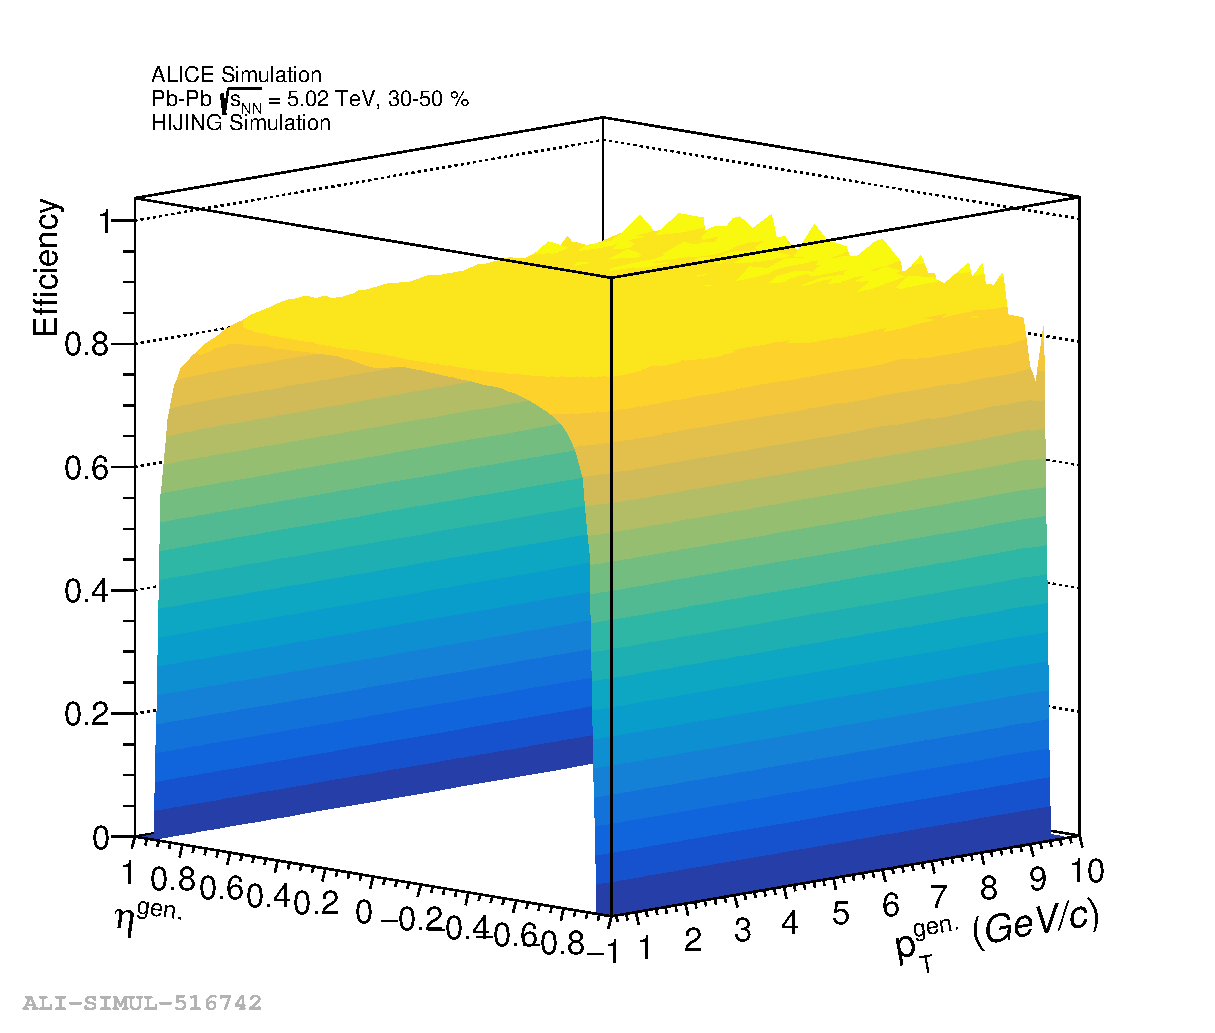
\includegraphics[width=0.8\textwidth]{figures/eps/Prelim_Approval_STRE_2.eps}
    \caption{Single track reconstruction efficiency as a function of $p_T$ and $\eta$ for Pb Pb collisions.}\label{fig:STRE}
\end{figure}

\subsection*{Pair Acceptance Efficiency}

The pair acceptance efficiency is defined as the probability that a jet-hadron pair will be reconstructed at a particular $\Dphi$, $\Deta$, jet $p_T$ and associated hadron $p_T$. In this analysis we use a mixed event technique to measure the pair acceptance efficiency. In this technique, we accumulate the hadrons in every event processed, forming a super event. Then, we compute the mixed event correlations between jets and the super event before adding the event containing the jet to the super event. These mixed event correlations, after normalization, are the pair acceptance efficiency. 

\subsubsection*{Mixed Events}

Mixed events are constructed by taking each event that is processed and adding all of its tracks to an event pool that is binned in event multiplicity and z-vertex position. A single track reconstruction efficiency is applied to the tracks that are added so that the resulting distribution is comparable to the raw correlations that have already been corrected for the single track reconstruction efficiency. Once an event pool contains a pre-specified minimum number of tracks, we calculate the correlations between jets in each remaining event and all tracks in the event pool with a matching multiplicity and z-vertex position. After normalizing the mixed event correlations distribution, described below, we divide the raw jet hadron correlations, corrected for single track reconstruction efficiency, by the mixed event correlations.

Before we can use the the mixed event correlation function as the pair acceptance efficiency, we need to normalize it. We assume that, once the single track reconstruction efficiency is applied, the mixed event correlation function will have its peak around $\Deta$ $\approx$ 0. This is because we have full acceptance in this region. This normalization can be done in several ways~\cite{EhlersThesis}. We use a sliding window approach over $\Dphi$. In order to perform the sliding window technique, we restrict our mixed event correlations to a small window in $\Deta$ where the mixed event correlations are roughly flat and project onto $\Dphi$. We used |$\Deta$| $\leq$ 0.3. We then compute the sliding average over $\Dphi$ using a window of size $\pi$/2 to determine the maximum of the un-normalized mixed event correlations. The sliding window average is less susceptible to statistical fluctuations than simply taking the maximum over $\Dphi$ After normalizing the mixed event correlations distribution, we divide the raw jet hadron correlations, corrected for single track reconstruction efficiency, by the mixed event correlations.

\subsection*{Background Estimation}

The background arises from many physical processes and has a different shape in p-p collisions as compared with Pb-Pb collisions. In p-p collisions, the background is relatively flat in ($\Dphi$, $\Deta$), allowing it to be modeled as a simple pedestal. In Pb-Pb collisions, the background is flat in $\Deta$, but not in $\Dphi$ and must be estimated from the data. The background is estimated from the region 0.8$\leq$ |$\Deta$| $\leq$ 1.2 and -$\pi$/2$\leq$ $\Dphi$ $\leq$ $\pi$/2. The procedures for estimating the background are described in the following sections.

\subsubsection*{p-p Background}

In p-p collisions, the background level is estimated by taking the average level measured in the background-dominated region defined by 0.8 $\leq$ |$\Deta$| $\leq$ 1.2 and -$\pi$/2$\leq$ $\dPhi$ $\leq$ $\pi$/2. This is done by integrating the jet-hadron correlation function over that region and dividing by the area of the region in ($\Dphi$, $\Deta$). 

\subsubsection{Pb-Pb Background}

In Pb-Pb collisions, the presence of flow result in azimuthal anisotropies in the background. We use the reaction plane fit(RPF) method to estimate the background in the presence of a flow-correlated background. The RPF method leverages the dependence of a jet on its angle with respect to the reaction plane to provide tangible formulas describing the flow-correlated background with respect to $\Dphi$. Because the background does not depend on $\Deta$, we integrate it out of the background dominated region,

\begin{equation}
    \rho_{bkg.}^{Corr.}(\Dphi) = \frac{1}{0.4}\int_{0.8}^{1.2}\rho^{Corr.}(\Dphi, \Deta) d\Deta + \frac{1}{0.4}\int_{-1.2}^{-0.8}\rho^{Corr.}(\Dphi, \Deta) d\Deta
\end{equation}

By fixing the angle of a jet to a range relative to the reaction plane, we can express the background as~\cite{RPF,RPF2}:

\begin{equation}
    b(\Dphi, \Psi^t) = \frac{dN^{pairs}}{\pi d\Dphi} = \tilde{\beta}(1+\sum_{n=1} 2 \tilde{v}_n^t \tilde{v}_n^a \cos(n\Dphi))
\end{equation}

where $\tilde{v}_n^t$, and $\tilde{v}_n^a$ are the jet and associated hadron effective $v_n$. $\tilde{\beta}$ is the effective background level given by,

\begin{equation}
    \tilde{\beta} = B (1 + \sum_{k=2,4,6,\etc} 2 v_k \cos(k \phi_s) \frac{\sin(kc)}{kc} R_k)
\end{equation} 

B is a fitting parameter controlling the level of the background, $R_k$ is the reaction plane resolution for the $k_{th}$ order reaction plane. $\phi_s$ is the center of the range that the jet azimuthal angle is fixed in and c is the width of that range. The effective $v_n$ for jets is given by,

\begin{equation}
    \tilde{v}_n^t = \frac{v_n+ \cos(n \phi_s) \frac{\sin(nc)}{nc}R_n + \sum_{k=2,4,6,\etc} (v_{k+n} + v_{|k-n|}) \cos(k \phi_s) \frac{\sin(kc)}{kc} R_k}{1+ \sum_{k=2,4,6,\etc} 2 v_k \cos(k \phi_s) \frac{\sin(kc)}{kc} R_k}
\end{equation}

We restrict our jet azimuthal angles to three regions relative to the reaction plane to constrain the RPF parameters: in-plane, mid-plane, and out-of-plane. The in-plane region is defined by $\phi_s$ = 0, c=$\pi$/6, and the out-of-plane region is defined by $\phi_s$ = $\pi$/2, c=$\pi$/6. The mid-plane region is defined by combining the regions with $\phi_s$ = $\pi$/4, c=$\pi$/12 and $\phi_s$ = 3$\pi$/4, c=$\pi$/12. 

We simultaneously fit all of these regions using the curve fit function from the python package scipy. The errors are computed by inverting the estimated Hessian matrix at the optimal parameter values, provided by curve fit. The fit parameters are B, $v_2^t$, $v_2^a$, ($v_3^t * v_3^a$), $v_4^t$, and $v_4^a$. The product of first-order flow coefficients, ($v_1^t * v_1^a$), is kept fixed at zero, due to the fact that $v_1^t$ is very likely zero and that fitting the interval -$\pi$/2 $\leq$ $\Dphi$ $\leq$ $\pi$/2 alone will not constrain its value. The result of allowing it to vary is that any value is acceptable and the other parameters will compensate erroneously. As a cross-check, the product was allowed to vary and the resulting optimal values were always within uncertainty of zero. The background-dominated region is restricted to the near-side with -$\pi$/2 $\leq$ $\Dphi$ $\leq$ $\pi$/2, and must be extrapolated to the away-side in order for background subtraction to be performed there. An estimate on the uncertainty due to the fitting procedure is computed from the covariance matrix produced by the fiting procedure.

\section{Particle Identification}

The TOF and TPC are used to identify particles in this analysis. We are ultimately interested in the particle fractions of identified particles in different regions of the jet-hadron correlations. We use these fractions to estimate the yields and ratios of each particle species in the near-side, away-side, and background regions. The particle fractions are estimated using the TPC dE/dx signal. The TPC signals for each species vary with associated hadron momentum and begin to overlap at moderate momenta, making it impossible to assign a clear species to each hadron. In order to estimate the particle fractions in each region, we use the TOF to help disentangle the species. The TOF provides a time-of-flight measurement for each particle, which can be used to help distinguish between different species, and is uncorrelated with the TPC signal. We use the TOF signal to sample each particle species preferentially, with varying levels of contamination. Then, we simultaneously fit the four resulting dE/dx distributions, one for each species: $\pi$, K, p, and one for the inclusive distribution. These fits are used to compute the particle fractions for each species in each region.

\subsection*{Particle Identification in the TPC}

The mean rate of energy loss as a particle traverses a gaseous volume is governed by the Bethe-Bloch formula~\cite{PDG}. The Bethe-Bloch formula is given by, 

\begin{equation}
    -\frac{dE}{dx} = K z^2 \frac{Z}{A} \frac{1}{\beta^2} \left[\frac{1}{2} \ln \frac{2 m_e c^2 \beta^2 \gamma^2 T_{max}}{I^2} - \beta^2 - \frac{\delta(\beta\gamma)}{2}\right]
\end{equation}

\noindent where K is a constant, z is the charge of the particle, Z is the atomic number of the material, A is the atomic mass of the material, $\beta$ is the velocity of the particle in units of the speed of light, $\gamma$ is the Lorentz factor, $T_{max}$ is the maximum kinetic energy that can be transferred to an electron in a single collision, I is the mean excitation energy, and $\delta$ is a density effect correction. Once the gas mixture is fixed, the formula is often parametrized according to the ALEPH parametrization:

\begin{equation}
    f(\beta\gamma) = \frac{P_1}{\beta^{P_4}} \left(P_2 - \beta^{P_4} - \ln\left(P_3+\frac{1}{(\beta\gamma)^{P-5}}\right)\right)
\end{equation}

\noindent where the parameters are measured once the detector is constructed and filled with the gas mixture. 

The specific energy loss per unit length as a function of momentum is shown for the TPC in Figure~\ref{fig:TPCdEdx}. At low momentum the signal provides clear separation between the species. As the momentum increases, the signal for different species begins to overlap, making it impossible to assign a clear species to each hadron. For each momentum bin, we take the dE/dx signal and compute the number of standard deviations away from the mean energy loss for a pion for each particle. We then model that distribution as a mixture of pions, kaons, and protons. Pions are distributed according to a Gaussian distribution with mean $\mu_{\pi}$ and width $\sigma_{\pi}$, which are expected to be near 0 and 1, but are allowed to float. Kaons and protons are distributed according to generalized Gaussians with a skewness parameter, $\alpha$. The overall mixture model is given as,

\begin{equation}
    f(x) = w_\pi \mathcal{N}(\mu_\pi, \sigma_\pi) + w_K \mathcal{G}(\mu_K, \sigma_K, \alpha_K) + w_p \mathcal{G}(\mu_p, \sigma_p, \alpha_p)
\end{equation}

\noindent where $w_\pi$, $w_K$, and $w_p$ are the fractions of pions, kaons, and protons, respectively. The parameters  $\mu_\pi$, $\sigma_\pi$, $\mu_K$, $\sigma_K$, $\alpha_K$, $\mu_p$, $\sigma_p$, and $\alpha_p$ are referred to as shape parameters and should depend only on the details of the TPC. The typical Gaussian distribution is given by,

\begin{equation}
    \mathcal{N}(\mu_\pi, \sigma_\pi) = \frac{1}{\sqrt{2\pi}\sigma_\pi}e^{-\frac{(x-\mu_\pi)^2}{2\sigma_\pi^2}},
\end{equation}

\noindent and the generalized Gaussian distribution is given by,

\begin{equation}
    \mathcal{G}(\mu, \sigma, \alpha) = \frac{1}{\sqrt{2\pi}\sigma}e^{-\frac{(x-\mu)^2}{2\sigma^2}}\left(\alpha \frac{x-\mu}{\sigma}\right)
\end{equation}

Mixture models are notoriously difficult to fit as they are nonconvex in nature. As a result, they depend heavily on the initial conditions of the fit. To mitigate this, we use extra information from the TOF to sample a biased population of each species, enhancing that species in the sample. We then fit the dE/dx distributions for each biased sample simultaneously. Because the TOF is uncorrelated with the TPC signal, the shape parameters should be shared amongst biased samples. Once the optimal shape parameters have been found they are fixed and the sample of particles with no TOF bias is fit to determine the particle fractions.

\subsection*{Particle Identification in the TOF}
